%%%%%%%%%%%%%%%%%%%%%%%%%%%%%%%%%%%%%%%%%%%%%%%%%%%%%%%%%%%%%%%%%%%%%%%%%%%%%%%%
%2345678901234567890123456789012345678901234567890123456789012345678901234567890
%        1         2         3         4         5         6         7         8

\documentclass[letterpaper, conference]{ieeeconf}  % Comment this line out if you need a4paper


% make changes take effect
\pagestyle{headings}
% adjust as needed
\addtolength{\footskip}{0\baselineskip}
\addtolength{\textheight}{-1\baselineskip}




%\documentclass[a4paper, 10pt, conference]{ieeeconf}      % Use this line for a4 paper

\IEEEoverridecommandlockouts                              % This command is only needed if 
                                                          % you want to use the \thanks command

% See the \addtolength command later in the file to balance the column lengths
% on the last page of the document

% The following packages can be found on http:\\www.ctan.org
\usepackage{graphicx} % for pdf, bitmapped graphics files
\usepackage{epstopdf}
%\usepackage{epsfig} % for postscript graphics files
%\usepackage{mathptmx} % assumes new font selection scheme installed
%\usepackage{times} % assumes new font selection scheme installed
\let\proof\relax
\let\endproof\relax
\usepackage{amsmath} % assumes amsmath package installed
\usepackage{amsthm}  % For special theorem style
\usepackage{amsfonts}
%\usepackage{amssymb}  % assumes amsmath package installed
\usepackage[dvipsnames]{xcolor}
\usepackage{tikz}
\usepackage{pgfplots}
\usetikzlibrary{shapes,arrows}
\usetikzlibrary{backgrounds}
\usepackage{multirow}
\usepackage[keeplastbox]{flushend}
%\usepackage{cite}  % Make sure that citation appear as [1]-[3] instead of [1], [2], [3]
\usepackage[utf8]{inputenc}    % utf8 support
\usepackage[T1]{fontenc}       % code for pdf file
\usepackage[style=ieee,doi=false,isbn=false,url=false,date=year,backend=biber,mincitenames=2,maxcitenames=2,mincitenames=1,uniquelist=false,uniquename=false,giveninits=true]{biblatex}
\renewcommand*{\bibfont}{\footnotesize}
\setlength{\biblabelsep}{\labelsep}
\bibliography{../bib}
\usepackage{pgfplots}
\pgfplotsset{compat=1.9}  % Prevent warning, pgf running in backwards compatibility mode anyway
%\usetikzlibrary{external}                       %% Create pdf figures from TikZ. Use PDFTeXify ...
%\tikzexternalize[prefix=tikz/]                  %% ... with --tex-option=--shell-escape switch.
\usepackage[capitalize]{cleveref}
\usepackage{subcaption}
\usepackage{xstring}
\usepackage{xparse}
\usepackage{units}
\usepackage{dblfloatfix}    % To enable figures at the bottom of page

\theoremstyle{plain}
\newtheorem{definition}{Definition}
\theoremstyle{remark}\newtheorem{remarkenv}{Remark}[section]        %% remarks
\newenvironment{remark}{\begin{remarkenv}}%
	{\hfill$\lozenge$\end{remarkenv}}            %% end remark with a lozenge

% Table stuff
\usepackage{booktabs}
\usepackage{tabularx}
\newcolumntype{Y}{>{\raggedright\arraybackslash}X}
\setlength{\heavyrulewidth}{0.1em}
\newcommand{\otoprule}{\midrule[\heavyrulewidth]}

%\pgfplotsset{compat=newest} 
%\pgfplotsset{plot coordinates/math parser=false}

%Images path 
\graphicspath{ {figures/} }


\title{\LARGE \bf
	Independent assessment strategy for autonomous vehicles
}


%\author{Erwin de Gelder$^{1*}$, Jan-Pieter Paardekooper$^{1}$, Arash Khabbaz Saberi$^{1}$, Hala Elrofai$^{1}$, Olaf Op den Camp$^{1}$, \\Bart De Schutter$^{2}$%
%\thanks{$^{1}$TNO, P.O. Box 756, 5700 AT Helmond, The Netherlands}%
%\thanks{$^{2}$Delft University of Technology, Delft Center for Systems and Control}%
%\thanks{$^{*}$Corresponding author. \newline E-mail address: {\tt\small erwin.degelder@tno.nl}}}%
\author{Erwin de Gelder, etc.}
%\thanks{*This work was not supported by any organization}% <-this % stops a space
%\thanks{$^{1}$Albert Author is with Faculty of Electrical Engineering, Mathematics and Computer Science,
%        University of Twente, 7500 AE Enschede, The Netherlands
%        {\tt\small albert.author@papercept.net}}%
%\thanks{$^{2}$Bernard D. Researcheris with the Department of Electrical Engineering, Wright State University,
%        Dayton, OH 45435, USA
%        {\tt\small b.d.researcher@ieee.org}}%


\newlength\figurewidth
\newlength\figureheight
\usetikzlibrary{arrows,positioning}
\usetikzlibrary{arrows.meta}
\definecolor{TNOblue}{RGB}{102,153,204}             %% TNO blue
\definecolor{TNOlightgray}{RGB}{222,222,231}

%\usepackage{changebar}
%\newcommand{\cbstart}{\color{blue}}
%\newcommand{\cbend}{\color{black}}
\newcommand{\todo}[1]{\color{red}TODO: #1\color{black}}

\usepackage{setspace}
%\doublespacing


\begin{document}


\maketitle
\thispagestyle{empty}
\pagestyle{empty}


%%%%%%%%%%%%%%%%%%%%%%%%%%%%%%%%%%%%%%%%%%%%%%%%%%%%%%%%%%%%%%%%%%%%%%%%%%%%%%%%
\begin{abstract}
	\todo{Write abstract}
\end{abstract}

%%%%%%%%%%%%%%%%%%%%%%%%%%%%%%%%%%%%%%%%%%%%%%%%%%%%%%%%%%%%%%%%%%%%%%%%%%%%%%%%
\section{Introduction}
\label{sec:introduction}

TODO

\color{red}
For Arash and Hala: please use \\{\tt \textbackslash cref\{sec:introduction\}}\\ to refer to sections, figures etc. It automatically adds things as `Section': e.g., \cref{sec:introduction}.
\color{black}

The introduction contains: 
\begin{itemize}
	\item Setting up the context of automated driving
	\item Giving some background information about the hazard analysis and risk assessment in the ISO~26262 standard
	\item The gap (the problem) We currently have this as a separate chapter, we could move it to introduction depending on the length. 
	\item our contribution. 
	\item paper structure
\end{itemize}
\section{Operational safety}
\label{sec:safety}

The ultimate goal of the assessment procedure is to determine whether a vehicle equipped with a level 4 or level 5 automation driving system (according to J3016 \cite{sae2018j3016}) is operationally safe. Therefore, before describing the assessment procedure, this section provides a brief overview of automotive safety notions and standards. 

The field of automotive safety is very broad, characterized by many types and definitions of the various aspects of safety. Nevertheless, on a high abstraction level, different types of safety are commonly distinguished, being \emph{functional safety}, \emph{cybersecurity}, \emph{safety of the intended functionality} (SOTIF). A fourth type of safety, being \emph{behavioural safety} can also be identified, relating to how the AV is programmed to behave. 

Functional safety, cybersecurity, SOTIF, and behavioural safety can be jointly referred to as \emph{operational safety}, as illustrated in \cref{fig:operational safety}. The four types of safety, as introduced here, are briefly explained in the next sections.

\begin{figure*}[b]
	\centering
	\tikzstyle{block}=[minimum width=8.5em, minimum height=4.5em, align=center, font=\small\sffamily, rounded corners=0.4em, fill=TNOlightgray]%
\begin{tikzpicture}
	%% Place the nodes
	\node[block](operational){Operational\\safety};
    \node[coordinate, below of=operational, node distance=7em](below operational){};
	\node[block, left of=below operational, node distance=5.2em](cyber){Cybersecurity};
	\node[block, left of=cyber, node distance=10.4em](functional){Functional safety\\(ISO~26262)};
	\node[block, right of=below operational, node distance=5.2em](sotif){SOTIF\\(ISO~21448)};
	\node[block, right of=sotif, node distance=10.4em](behavioural){Behavioural safety};
	
	%% Place the lines
	\node[coordinate, below of=operational, node distance=3.5em](operational helper){};
	\draw (operational) -- (operational helper) -| (functional);
	\draw (operational) -- (operational helper) -| (cyber);
	\draw (operational) -- (operational helper) -| (sotif);
	\draw (operational) -- (operational helper) -| (behavioural);
\end{tikzpicture}

	\caption{In this paper, we distinguish four aspects of operational safety: Functional safety, cybersecurity, safety of the intended functionality (SOTIF), and behavioural safety.}
	\label{fig:operational safety}
\end{figure*}



\subsection{Functional safety}
\label{sec:functional safety}

Functional safety is defined in IEC~61508 as the absence of unacceptable risk due to hazards caused by malfunctioning behaviour of systems. ISO~26262 \cite{ISO26262}, commonly referred to as ISO~26262, is an adaptation of the IEC~61508 for the automotive industry. It applies to safety-related electrical/electronic systems, specifically for road vehicles under \unit[3500]{kg}.

The ISO~26262 standard that was introduced in 2011 does not include automated vehicles. Advanced driver assistance systems (ADAS) are, however, included in the next release of ISO~26262 in 2018 \cite{ISO26262}. In ISO~26262, the notion of functional safety has been defined as follows.

\begin{definition}[Functional safety \cite{ISO26262,Dubey2017}] \label{def:functional safety}
	Functional safety is the absence of unreasonable risk due to hazards caused by malfunctioning behaviour of electrical/electronics systems.
\end{definition}

In \cref{def:functional safety}, risk refers to the combination of occurrence of harm and the severity of that harm. The malfunctioning behaviour refers to a failure or unintended behaviour of the system. According to this definition, functional safety is `looking inwards', focusing on malfunctioning AV components. 

ISO~26262 provides a guidelines from concept phase to production phase of an so-called item; that is, a system or an array of systems. This is helpful for internal safety assessment --- for development organizations --- and external safety assessment --- for independent organization. Since this work aims to provide an assessment framework for an independent assessor, it focusses especially on the start and the end of the development. This is shown in \cref{fig:ISO26262}, where an overview of ISO~26262 is presented and the focus of this work using the blue rectangles. The assessment focusses on the overall safety management, the concept phase, and the safety validation. In the remaining of this section, we will describe in more detail these parts of ISO~26262

\begin{figure*}[t]
	\centering
	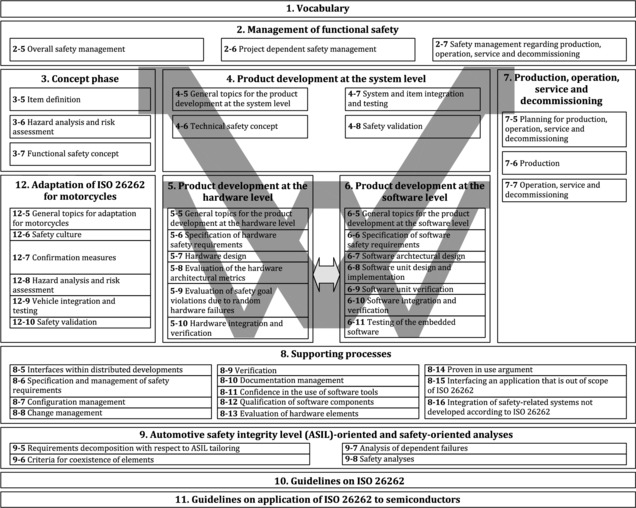
\includegraphics[width=.825\textwidth]{ISO26262_2018.png}
	\tikz[overlay]{\node[minimum height=5.2mm, minimum width=45mm, draw=TNOblue, ultra thick, rounded corners=0.4mm] at (-12.29,10.53) {};
	\node[minimum height=17.8mm, minimum width=32.5mm, draw=TNOblue, ultra thick, rounded corners=0.4mm] at (-12.95,8.8) {};
	\node[minimum height=5.7mm, minimum width=30.4mm, draw=TNOblue, ultra thick, rounded corners=0.4mm] at (-5.3,8.8) {};}
	\caption{An overview of ISO~26262. The blue rectangles denote the relevant parts for this work. The figure is based on \cite{ISO26262}.}
	\label{fig:ISO26262}
\end{figure*}

% Comment [Erwin]: Text is omitted, since it is not up to date. The safety lifecycle in the newest ISO 26262 from 2018 looks significantly different.
%The process that must be followed according to the ISO\,26262 to arrive at a functionally safe system design, the so-called `safety lifecycle', is shown in \cref{fig:ISO26262}. In the scope of AV safety assessment, the validation processes included in this lifecycle (indicated by the blue boxes in the figure) are particularly relevant; These are briefly summarized as follows.
%
%\begin{figure}[tb]
%	\centering
%	\includegraphics[width=\textwidth]{safety_lifecycle.png}
%	\tikz[overlay]{\node[minimum height=17mm, minimum width=30mm, draw=TNOblue, ultra thick, rounded corners=0.4mm] at (-0.25,8.14) {};
%		\node[minimum height=15.7mm, minimum width=31.1mm, draw=TNOblue, ultra thick, rounded corners=0.4mm] at (-0.19,4.17) {};}
%	\caption{The ISO~26262 safety lifecycle (extracted from \cite{ISO26262}).}
%	\label{fig:ISO26262}
%\end{figure}

The overall safety management of the organization developing the AV is of particular interest, because the organization and management directly impacts the functional safety of the AV \cite{yaping2019safetydriven}. In fact, the nature of safety culture is already addressed for decades in all kinds of industries \cite{choudhry2007nature}. The safety management also addresses the safety culture, which is, according to \textcite[p.~5]{piers2009safety}, defined as ``the set of enduring values and attitudes regarding safety, shared by every member of every level of an organization.'' The safety culture is typically measured through interviewing the staff. \textcite{carroll1998safety} performs a qualitative measurement of the safety culture of a departments at a nuclear power plant that reveals some issues with the safety and work culture. Therefore, such a qualitative measurement of the safety culture can positively influence the safety culture when all issues are appropriately addressed. \textcite{warszawska2016method} propose a quantitative estimation of the level of safety culture in an organization. They argue that the presented algorithm could be successfully applied in different types of the organization. \textcite{khabbazsaberi2018method} propose a method for quantitative measurement of the safety culture based on ISO~26262. Therefore, their approach might be most applicable for measuring the overall safety management of the organization developing the AV.

According to ISO~26262, the concept phase consists of three steps: the item definition, the hazard analysis and risk assessment (HARA), and the functional safety concept. Whereas the item can refer to a function of the vehicle, in our case it is referring to the AV as a whole. The objective of the item definition is ``to define and describe the item, its dependencies on, and interaction with, the environment and other items; and to support an adequate understanding of the item so that the activities in subsequent phases can be performed'' \cite[Clause 3.5]{ISO26262}. A crucial element of the item definition is the definition of the operating conditions since the AV is unlikely to operate under all conditions \cite{koopman2016challenges}. The item definition is an important input for the assessment and, therefore, the vehicle, the ODD, and the DDT need to be defined when applying for the assessment.

The objective of the HARA is ``to identify and to categorise the hazardous events caused by malfunctioning behaviour of the item; and to formulate the safety goals related to the prevention or mitigation of the hazardous events, in order to avoid unreasonable risk'' \cite[Clause 3.6]{ISO26262}. Using a HARA to assess the risks is already done for decades \cite{sage1980methodologies}. \textcite{johansson2015importance} discusses the use of a HARA for AVs and, especially, the completeness of the HARA. \textcite{johansson2015importance} further argues that elaborating the HARA --- instead of defining only few general safety goals --- results in a potential to significantly save costs because of the large implications of general safety goals on the whole AV. For an example of an HARA for an AV, see \cite{stolte2017hara}. As part of the HARA, the hazards are categorised according to the Automotive Safety Integrity Level (ASIL). The ASIL is based on qualitative scores for the severity (the estimate of the extent of harm), the controllability (the ability to avoid a specified harm or damage), and the probability of exposure (the state of being in an operational situation). The ASIL determines to what extent certain measures need to be taken to minimize a risk. Since the ASIL is based on qualitative experts' judgements, it is not always reliable \cite{khastgir2017towards}. As such, several attempts are made to make the HARA more objective; for example using a rule-set for determining the scores of the severity, controllability, and exposure \cite{khastgir2017towards}. \textcite{duracz2015rigorous} use simulations to support the HARA. Another possibility is to use real-life driving data and simulations to arrive to a quantitative measure for risk \cite{degelder2019risk}.

The functional safety concept \cite[Clause 3.8]{ISO26262} involves specification of functions and their interactions which are necessary to achieve the desired safe behaviour as defined by the safety goals resulting from the HARA. 

\todo{Check whether the functional safety concept should be part of this report. Do we assess the functional safety concept? I (Erwin) cannot see it immediately in the document review.}

The safety validation checks, on a vehicle level, whether the safety goals are fulfilled. This is done through virtual and physical testing, representing the `intended use cases', i.e., the traffic scenarios as they occur in the envisioned operational environment of the AV.

\begin{remark}
	Intuitively, one might think that (safety) \emph{verification} is more appropriate to indicate the main assessment objective. ISO\,26262, however, defines verification as ``determination of completeness and correct specification, or implementation, of requirements from a phase or sub-phase,'' which clearly makes this notion less suitable to express the assessment objective.
\end{remark}

%When adopting the selected topics of the lifecycle, a first step is made towards a process for safety assessment of AVs from the perspective of functional safety; This is visualized in \cref{fig:functional safety assessment}, where the scenario generation component, which is not explicitly included in the original ISO process, aims to generate relevant traffic scenarios (either or not as part of overarching `use cases').
%
% Erwin: I removed figure, because I do not see the added value (anymore)
%\begin{figure}[tb]
%	\centering
%	\includegraphics[scale=1]{functional_safety_assessment.pdf}
%	\caption{Functional safety assessment steps, inspired by the ISO~26262.}
%	\label{fig:functional safety assessment}
%\end{figure}

%From the information presented in this section, it can be concluded that the ISO~26262 standard is oriented towards development of a certain automation functionality, as part of which verification and validation processes are implemented. The objective of the assessment pipeline, however, is not to design a safe AV but to assess the safety of a given design. Consequently, the process from \cref{fig:functional safety assessment} needs to be further adapted, both in terminology and in contents, to better fit this objective. The next chapter (in particular \cref{sec:document review}) will further specify the role of the safety validation process in the assessment procedure, as a start for further development of the pipeline.


\subsection{Cybersecurity}
\label{sec:cybersecurity}

Whereas functional safety focusses on hazards caused by malfunctioning behaviour of components \emph{inside} the vehicle, cybersecurity focusses on threats from \emph{outside} the vehicle. Cybersecurity is a broadly used term and many different definitions exist; see \cite{craigen2014defining} for an overview of existing definitions. TR68-3 \cite[p.~9]{tr68cybersecurity} defines cybersecurity as ``the protection of electronic systems from cyberattacks'', where a cyberattack is defined as ``an assault on an electronic system to violate its confidentiality, integrity, or availability through cybersecurity means [...]'' \cite[p.~9]{tr68cybersecurity}. \textcite[p.~1]{lewis2006cybersecurity} writes that ``cybersecurity entails the safeguarding of computer networks and the information they contain from penetration and from malicious damage or disruption.'' Throughout this work, we adopt the definition from \textcite{craigen2014defining}, which resulted from an in-depth literature review and multiple discussions on cybersecurity with practitioners, academics, and graduate students:

\begin{definition}[Cybersecurity \cite{craigen2014defining}]
	Cybersecurity is the organization and collection of resources, processes, and structures used to protect cyberspace and cyberspace-enabled systems from occurrences that misalign \textup{de jure} from \textup{de facto} property rights.
\end{definition}

AVs will be increasingly connected; for example using vehicle-to-vehicle and vehicle-to-infrastructure communications and Internet of Things devices connected to the vehicle, such as bluetooth-connected mobile phones. With respect to cyber attacks, a connected device means an exposed device. As such, an autonomous vehicle is a highly exposed device that relies heavily on its hackable software. Cybersecurity needs to be considered as the cyber attacks may lead to major safety losses \cite{hashemeiza2017sharks}.

Because of the many connections an AV has with its outside world, there are many cyber threats. The driving behaviour can be controlled by attacked the internal bus system of an AV \cite{wolf2004security}, possibly through the on-board diagnostics port that every modern car has \cite{checkoway2011comprehensive}. Vehicle-to-vehicle communications using dedicated short range communications are exposed to, amongst others, denial-of-service attacks \cite{lyamin2014real} and false messages \cite{moalla2012risk}. Since the AV depends on its software, it is vulnerable to malware attacks \cite{zhang2014defending}. Connected a vehicle to a mobile device introduce other security challenges \cite{yan2015twoyear, oka2014bluetooth}. Because an AV heavily relies on its sensors, it is also exposed to spoofing attacks \cite{yan2016can, davidson2016controlling}, which utilizes the underlying principles of sensors to blind or deceive them. For an overview of different cyber threats, see \cite{cui2018review, hashemeiza2017sharks, studnia2013survey, yaugdereli2015study, vanderheijden2016survey, sakiz2017survey, zheng2016investigating}. 

TR68-3 \cite[p.~12]{tr68cybersecurity} lists four key cybersecurity principles, ``referenced and in-line with industry best practices'', which are security by design, defence in depth, continuous operational management and oversight, and resiliency. Security by design \cite{ross2018systems, chattopadhyay2018autonomous} means that the cybersecurity implementation is considered from the start of the design of the product, rather than addressing specific attacks in an isolated and ad-hoc manner. This also includes formal validation and verification steps prior to the release of the product. Defence in depth, also referred to as Castle Model \cite{leuprecht2016beyond}, requires a holistic approach to cybersecurity built into all layers of the system architecture to ensure integrated and comprehensive protection of the entire system. Continuous operational management and oversight includes the prediction of potential threats \cite{gandotra2015computational}, the detection of attacks, and effective responds to attacks. Whereas cybersecurity mostly focusses on known attacks, cyber resilience is about ensuring that the system is prepared for the event of an unforeseeable and unpredictable attack \cite{sharkov2016cybersecurity}.

%\begin{itemize}
%	\item \emph{Security-by-design}: This means that the cybersecurity implementation needs to be systematic and process-oriented. Furthermore, it includes formal validation and verification steps prior to product release.
%	\item \emph{Defence-in-depth}: This requires a holistic approach to cybersecurity built into the system architecture to ensure integrated and comprehensive protection of the entire system.
%	\item \emph{Continuous operational management and oversight}: The cybersecurity operations need to be continuously operational and include predicting potential threats, detecting attacks, and responding effectively.
%	\item \emph{Resiliency}: Resiliency is about ensuring that cybersecurity preparedness and readiness is in place ready for the event of an incident.
%\end{itemize}

\subsection{Safety of the intended functionality}
\label{sec:sotif}

\todo{Link section with TR68-2. Provide more references.}

As mentioned earlier, functional safety is `inward looking', in the sense that it focuses on malfunctioning AV components, which include the vehicle platform, sensors and automation system. For AVs, however, it is also important to `look outwards', i.e., to include inherent sensor and perception system limitations in the safety assessment framework and to take decision-making capabilities of the AV into account. These aspects of AV safety are covered by the notion of \emph{safety of the intended functionality} (SOTIF).

SOTIF relates to hazardous behaviour which is not caused by a malfunction. In particular for AVs, SOTIF is often related to environmental perception \cite{Fischer2017} since environmental sensors typically have inherent limitations, which may cause the AV to behave unsafely. Examples of such limitations are the occurrence of so-called `ghosts' in radar measurements, or the blinding effect of direct sunlight in case of camera systems. It is important to mention that SOTIF is assessed on a system level, as opposed to functional safety, which is focusing on the AV component level. This type of safety is described in the standard ISO/WD\,PAS\,21448, in short referred to as ISO\,21448, which is currently under development \cite{ISO21448}. This draft standard defines SOTIF in a very broad sense as ``the absence of unreasonable risk of the intended functions''. In the scope of the current document, a more precise definition will be adopted, as proposed below. 

\begin{definition}[Safety of the intended functionality]
	Safety of the intended functionality (SOTIF) is the ability of the automation system to correctly comprehend the environmental situation and behave safely, by ensuring that the AV systems and components are operating within their design boundaries and, if they are not, by activating appropriate countermeasures.
\end{definition}

\subsection{Behavioural safety}
\label{sec:behavioural safety}

\todo{Link section with TR68-1. Provide more references.}

Whereas ISO\,21448 intends to facilitate safe functionality and ultimately provide sufficiently detailed and robust object and event detections, there is another type of safety that involves using these detections to correctly interpret the traffic situation and subsequently safely discharge manoeuvre planning. This can be captured by the notion of \emph{behavioural safety}, which, in a recent report by Waymo \cite{Waymo2017}, is introduced as ``An aspect of system safety that focuses on how a system should behave normally in its environment to avoid hazards and reduce the risk of mishaps: for instance, detect objects and respond in a safe way (slow down, stop, turn, lane change, etc.).'' This type of safety thus addresses the AV behaviour as intentionally programmed by the developer, with all components and systems of the AV operating as intended. A relevant question in this context is, for instance, whether the AV follows the traffic rules. Since it is questionable whether this type of safety will be part of the final version of ISO\,21448, behavioural safety is regarded as a third type of safety.

The UN-ECE Automatically Commanded Steering Function group is drafting amendments to UN-ECE Regulation 79 which describes the expected behaviour of a level 3 automated driving system \cite{sae2018j3016}. However, the scope is limited to well-structured and controlled highways where there are no pedestrians/bicycles, at least two lanes in the direction of travel, and a physical separation between contraflow traffic. The authors are not aware of existing art describing the behavioural safety requirements for a level 4 automated driving system operating in complex urban environments, hence this study aims to provide some definition to the behavioural characteristics required for a vehicle using the context of Singapore's road traffic rules and traffic environment as the case study. The proposed assessment methodology makes use of traffic scenarios to assess the behavioural safety of the AV. The safety assessment procedure, which is described in \cref{sec:assessment}, sets out how the scenarios are defined from a Document review exercise and from scenario generation using acquisition of real-world driving data. Next, the AV's behavioural performance is assessed through virtual and physical safety validation using these scenarios.

\section{Nomenclature} % Erwin (use the other paper) & Arash
\label{sec:definitions}

TODO: give more examples
First, we introduce the following notions:
\begin{enumerate}
\item Risk = Severity $\times$ Probability
\item Severity: a quantitative measure, depending on the impact velocity.
\item Condition:
\item Actor: the relevant actors here are the lead vehicle (denoted with L), the following vehicle (F) and the communication unit (V2V)
\item Activity: the relevant actions here are braking, and failure.
\item Scenario:
\end{enumerate}

\section{Procedure for the safety assessment}
\label{sec:procedure}

This paper assumes that many of the relevant tests for the safety assessment are performed in a virtual simulation environment that is controlled by the applicant. The proposed procedure intends to consider all results, both from virtual simulation and from actually performed physical tests. Where the assessor does not have access to the required models of the AV under test, the assessor will have the capability to perform physical tests on the AV. How to balance between the different results in the assessment, considering virtual and physical test results of the applicant and physical test results of the assessor is schematically presented in \cref{fig:procedure}. Each rectangular block represents an action. The procedure distinguishes between actions for which the applicant is responsible and actions for which the assessor is responsible. The procedure consists of the following actions:
\begin{enumerate}
	\item The first action is to derive which system-level tests need to be performed with reference to the ODD and DDT of the AV under test. Here, “system-level” is mentioned explicitly, because it is assumed that also in case of a failure of any of the subsystems, the AV would fail the system-level tests. Note, however, that it is advised that the applicant ensures that each of the subsystems underwent a rigorous assessment before applying for the AV assessment. 
	\item If the derived tests are acceptable, the next action is to select the tests for the assessment. Here, a distinction is made between tests for which the applicant is fully responsible and physical tests that are conducted by the assessor. The latter will focus more on spot checking.
	\item Once the tests are selected, these tests need to be conducted. The results of these tests will be described using prescribed metrics. Note, however, that these metrics may not contain too much information as it is assumed that the applicant does not want to disclose details of sensor and system implementation or even detailed test results because of the proprietary or confidential information contained in these results. 
	\item The final step is to assess the results from the tests and to formulate an advice for the authority on whether the AV is ready for deployment and under which conditions.
\end{enumerate}

\begin{figure*}
	\centering
	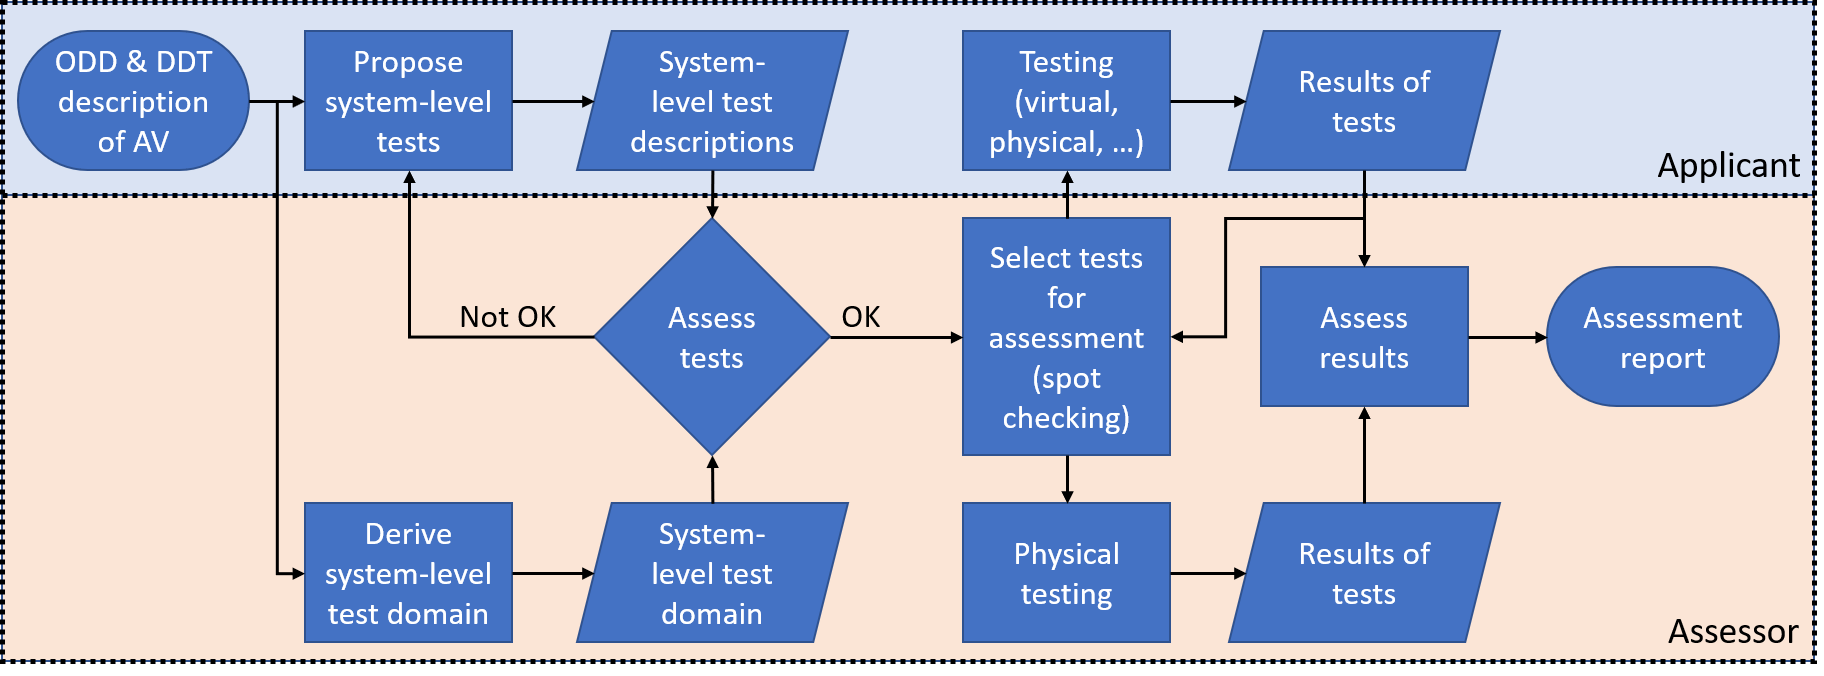
\includegraphics[width=\linewidth]{figures/procedure}
	\caption{Proposed framework for the safety assessment of an autonomous vehicle (AV).}
	\label{fig:procedure}
\end{figure*}

In the following sections, each of the actions are further detailed. We end this section with a short note on monitored deployment in case of a successful completion of the assessment.



\subsection{Deriving test descriptions}
\label{sec:test descriptions}

Based on the ODD and the DDT of the AV, the tests are derived. Following the same reasoning as \textcite{stellet2015taxonomy}, a test is an evaluation of:
\begin{itemize}
	\item a statement on the system-under-test (test criteria; what are we going to evaluate using the test);
	\item under a set of specified conditions (test case; how are we going to evaluate the test criteria);
	\item using quantitative measures (metrics; how to express the outcome of the test quantitatively);
	\item and a reference of what would be the acceptable outcome (reference; when is the outcome acceptable).
\end{itemize}

Since the applicant has designed and developed the AV, it is expected that the applicant has a clear notion of the tests that are required for a complete assessment of the AV and which the AV should appropriately handle. Similarly, if the set of relevant test descriptions is not complete during the development of the AV, it is conceivable that the AV will not operate safely for all circumstances possible within the ODD. 

Although it is expected that the applicant provides all relevant test descriptions, it is important that the applicant and the assessor discuss these test descriptions, and that a check is made whether or not the test descriptions are complete and cover the ODD sufficiently. If an important test description is missing, it is conceivable that the AV is not specifically designed to pass the corresponding test. In order to assess the completeness of the test descriptions provided by the applicant, the assessor needs to define the test domain for the relevant system-level test descriptions and use these to investigate if any important test descriptions are missing. Here, the so-called test domain refers to a more high-level description of the range of tests that are expected, rather than an enumeration of the large number of relevant tests.

If it turns out that the test descriptions that are provided by the applicant are not complete, the process needs to be restarted, as indicated by the ``Not OK'' line in \cref{fig:procedure}. On the other hand, if the test descriptions are deemed to be complete enough, the assessment proceeds to the next step: selecting tests for the assessment.



\subsection{Selecting tests for the assessment}
\label{sec:selection}

In principle, the applicant is expected to provide results for all tests. In the next section, we explain how these results may look like. Based on these results, tests are selected for the physical testing performed by the assessor. This is indicated by the arrow pointing from ``results of tests'' of the applicant to ``select tests for assessment'' in \cref{fig:procedure}.  

A test is selected for physical testing by the assessor if any of the following three statements are true:
\begin{itemize}
	\item The applicant does not provide a result. Although the applicant is expected to provide results for most tests, it might be possible that there are some tests for which the applicant does not have the resources to perform the tests reliably, for example if specific tooling is required. Note, however, that if the applicant does not provide results for too many tests, the assessment automatically results in a fail.
	\item The result seems inconsistent. If there is sufficient reason for the assessor to not confide in the result provided by the applicant, the test can be performed by the assessor to check the result provided by the applicant.
	\item The test is selected for spot checking. The main reason to perform spot checking is to assess the fidelity of the results provided by the assessor.
\end{itemize}
The process of test selection is summarized in \cref{fig:selection}.

\begin{figure}
	\centering
	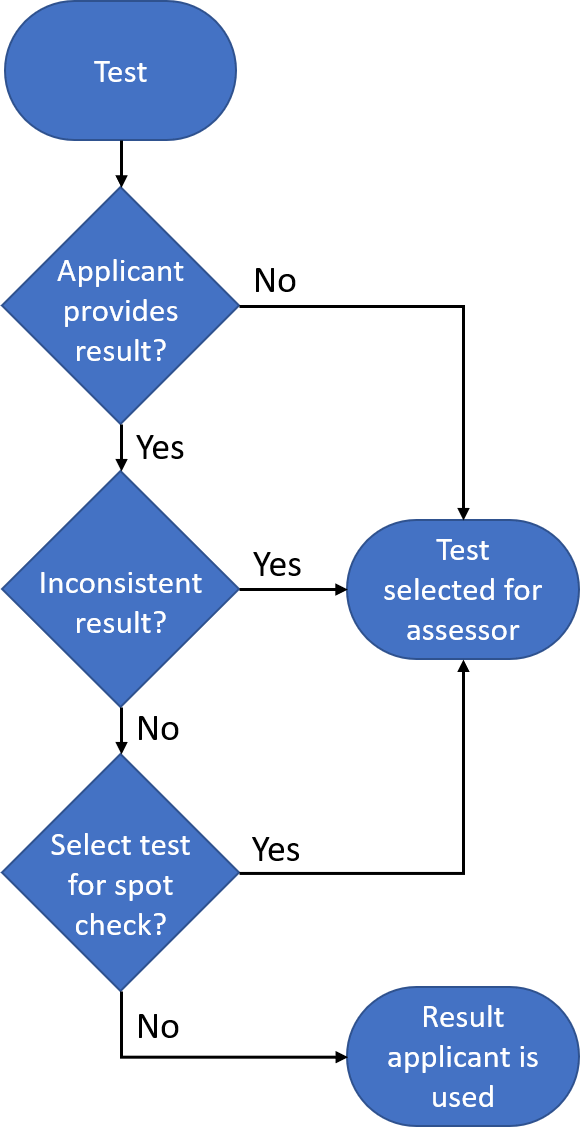
\includegraphics[width=.65\linewidth]{figures/test_selection}
	\caption{Decision scheme for the selection of a test for physical assessment by the assessor.}
	\label{fig:selection}
\end{figure}



\subsection{Testing}
\label{sec:testing}

As explained in the previous section, the applicant is expected to provide results for most tests. However, it is assumed that the applicant does not want to disclose detailed test results. Therefore, a rating scheme is proposed. Using a specific metric for each test, three references are defined: an acceptable result, a fair result, and a good result. If the result of the test is worse that the acceptable result, a ``fail'' is reported. If the result passes the acceptable reference but not the what is defined as a fair result, an ``acceptable'' is reported. Similarly, a ``fair'' is reported if the result is between a fair and a good result. If the result is better than what has been defined as a good result, a ``good'' is reported. This is schematically shown in \cref{fig:rating}. 

\begin{figure}
	\centering
	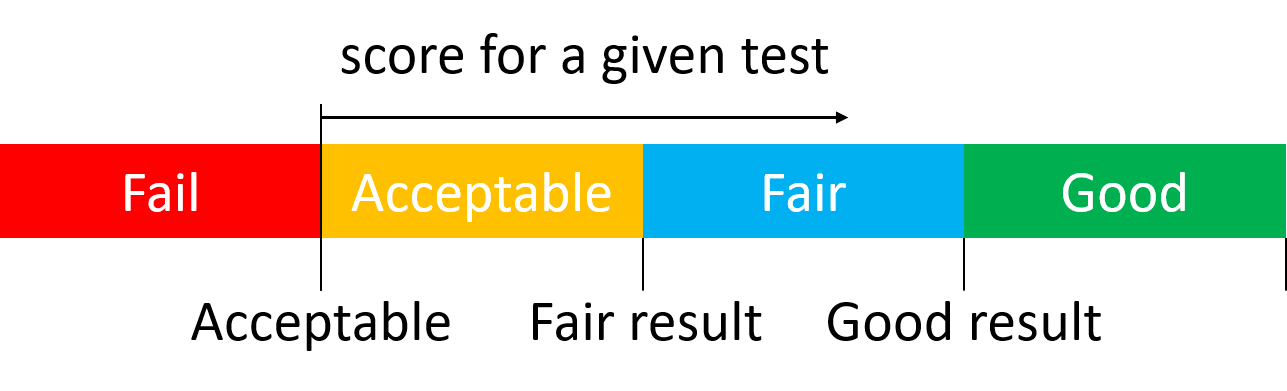
\includegraphics[width=\linewidth]{figures/rating}
	\caption{Different scoring options per test.}
	\label{fig:rating}
\end{figure}

In principle, the applicant is free to choose any method to derive the results. However, considering the large number of tests, the use of virtual simulations seems inevitable. In practice, it is expected that a both virtual simulations, physical tests, and a combination, such as hardware-in-the-loop testing, is used to determine the test results.

On the other hand, the tests by the assessor are performed physically. The main reason for this is that virtual simulations are ruled out as that would require the applicant to provide a model of the AV, which is expected to be impossible because of proprietary reasons.



\subsection{Assess results}
\label{sec:assess results}

The following assessment results are distinguished per test:
\begin{itemize}
	\item In case the test results show that for the specific test the AV performs acceptable (i.e., ``acceptable'', ``fair'', or ``good'', see \cref{fig:rating}), the test is passed. If this is not the case, then the specific test fails.
	\item Inspired by ISO~9001 on quality management \autocite{ISO9001}, a passed test may result in a non-conformity. An “acceptable” result automatically leads to a non-conformity (NC). This means that the response of the AV deviates substantially from  response that is qualified as “good”, but the deviation is not severe. Since the AV meets the minimum requirement for this test and consequently safety is not compromised, there is no reason to fail the AV based on this test. Nevertheless, an NC is issued to indicate that the applicant is asked to consider improvements, e.g., for a next version of the system.
	\item In case the test is also performed by the assessor and the corresponding result is worse than the reported result of the applicant, this also leads to a NC.
	\item The assessment of a test result might come with an observation (OB) that needs consideration of the applicant. 
\end{itemize}

If a test results in a fail, then either the assessment results in a negative advice of the assessor to the authority or it is advised to only allow for deployment of the AV under certain conditions. For example, if the only tests that are failed consider low-light conditions, the AV might be deployed under the condition that it operates only from sunrise till sunset. 

NCs and OBs do not lead to an immediate fail of the assessment. However, it is likely that they lead to a fail in a future assessment, e.g., when test criteria become increasingly demanding, and the applicant does not appropriately consider such NCs or OBs. NCs provide information to the applicant on how requirements might develop in the future, which, consequently, gives direction and motivation on continuous improvement of AVs regarding safety. On the other hand, many NCs – the AV barely passes the test in many cases – might mean that safety is compromised and, therefore, it might also result in a negative advice of the assessor to the authority regarding the deployment of the AV.

Note that when many NCs are observed, the AV probably will not be able to pass all tests if all tests would be performed physically by the assessor. Theoretically, this is however still possible. To minimize the risk of having an AV that passes all tests, but with many NCs, a system using demerit points is introduced. The AV starts with, e.g., 100 points, and in the assessment, 1, 2, or 3 points are subtracted for each NC, depending on the severity of the NC. Once the number of points for the AV are reduced to 0, then the AV is indicated to have failed he assessment because of an overrun of NCs. The numbers given here are merely provided as an example.



\subsection{Monitored deployment}
\label{sec:monitored deployment}

A successful completion of the proposed assessment might result in the approval for the deployment of the AV under the condition that the behavior of the AV on the road is continuously monitored. We propose that during such a deployment phase, the applicant is required to upload detailed driving data to allow for monitoring the AV behavior. This is implemented for two reasons:
\begin{itemize}
	\item After completion of the assessment pipeline, road and/or vehicle authorities may require the monitoring of safety continuously when driving on the public road.
	\item The uploaded data may be used to improve the generation of tests and the selection of relevant test cases for a particular AV, as is possible that some tests have been overlooked during the initial assessment process or that situations on the road gradually change with changes in traffic, e.g.because of the introduction of new mobility systems.
\end{itemize}

The feedback to the data acquisition element allows for ongoing learning and improvement of the standards and assessment systems, while being able to adapt to new types of transportation such as personal mobility devices. For example, additional test cases could be identified and incorporated into future safety assessment procedures. A deployment might consider new operational areas, the extension of the scenario database with scenarios that potentially differ between such areas would then be covered. Moreover, to obtain a scenario database that is `complete', i.e., statistically accurate, it is expected that operational data collection is required over an extended period, which most probably will not be realized before the deployment is operationalized. In other words, the imperfection of the assessment framework should not become a barrier for the introduction of new safe mobility solutions onto the market, in case these devices are tested to be safe for all currently known conditions. The assessment method, especially the step regarding monitored deployment, supports the continuous increase in knowledge on the state-of-the-art of road safety and herewith prepares the safety assessment method to be sustainable for the future.

%\section{Ontology for scenarios}
\label{sec:ontology}

We have already explained the use of an ontology in \cref{sec:why ontology}. In this section, we present our ontology for scenarios for the assessment of automated vehicles. 
The ontology is formally represented through a domain model that is briefly presented in \cref{sec:domain model}. Next, in \cref{sec:domain scenario category}, we explain how a scenario category is formally represented using the domain model. Similarly, in \cref{sec:domain scenario}, we describe how a scenario is formally represented using the domain model. 
%For more details on the domain model that is representing the ontology, see \cref{sec:appendix domain model}.



\subsection{Domain model}
\label{sec:domain model}

The classes of the domain model that are used to define a scenario and a scenario category are shown in \cref{fig:ontology classes}, where each block represents a class\cbstartd\footnote{\cbstartd In the remainder of this paper, when referring to (an instance of) a class, italic font is used.\cbend}\cbend.
The blue blocks represent the classes that are used to qualitatively describe a scenario whereas the orange blocks represent the classes that are used to quantitatively describe a scenario. 

\begin{figure}
	\centering
	\definecolor{scenarioclass}{RGB}{30, 144, 255}
\definecolor{category}{RGB}{0, 191, 255}
\definecolor{scenario}{RGB}{255, 69, 0}
\definecolor{otherclass}{RGB}{255, 127, 80}
\newlength\blockwidth
\newlength\blockheight
\newlength\blockx
\newlength\blocky
\newlength\legendwidth
\setlength{\blockwidth}{5.3em}
\setlength{\blockheight}{4em}
\setlength{\blockx}{6.4em}
\setlength{\blocky}{-7em}
\setlength{\legendwidth}{3.5em}
\tikzstyle{class}=[draw, text width=\blockwidth-.5em, align=center, minimum height=\blockheight, line width=1pt, minimum width=\blockwidth]
\tikzstyle{aggregation}=[-{Diamond[width=8pt, length=12pt, fill=white]}, line width=1pt]
\tikzstyle{falls into}=[->, line width=1pt]
\tikzstyle{superclass}=[-{Triangle[width=8pt, length=12pt, fill=white]}, line width=1pt]
\begin{tikzpicture}
% Classes
\node[class, fill=scenarioclass](scenario class) at (.5\blockx,0) {Scenario class};
\node[class, fill=category](staticcategory) at (\blockx, \blocky) {Static environment category};
\node[class, fill=category](activitycategory) at (2\blockx, \blocky) {Activity category};
\node[class, fill=category](model) at (1.5\blockx+0.25\blockwidth, 2\blocky) {Model};
\node[class, fill=category](actorcategory) at (3\blockx, \blocky) {Actor category};
\node[class, fill=scenario](scenario) at (.5\blockx, 2\blocky) {Scenario};
\node[class, fill=otherclass](static) at (\blockx, 3\blocky) {Static environment};
\node[class, fill=otherclass](activity) at (2\blockx, 3\blocky) {Acitivity};
\node[class, fill=otherclass](actor) at (3\blockx, 3\blocky) {Actor};
\node[class, fill=otherclass](triggered) at (1.5\blockx, 4\blocky) {Triggered activity};
\node[class, fill=otherclass](detected) at (2.5\blockx, 4\blocky) {Detected activity};

% Aggregation arrows for the scenario class
\node[coordinate, below of=scenario class, node distance=-\blocky/2, xshift=\blockwidth/3](helper scenario class){};
\node[coordinate, below of=scenario class, node distance=\blockheight/2, xshift=\blockwidth/3](aggregation scenario class){};
\foreach \class in {static, activity, actor}
{
	\node[coordinate, above of=\class category, node distance=\blockheight/2](helper \class){};  % Needed for later
	\draw[aggregation] (\class category) |- (helper scenario class) -- (aggregation scenario class);
}
\node[anchor=south east] at (helper static) {1};
\node[anchor=south east] at (helper activity) {$\mathbb{N}$};
\node[anchor=south east] at (helper actor) {$\mathbb{N}$};

% Aggregation arrow for the model
\node[coordinate, above of=model, node distance=\blockheight/2, xshift=-\blockwidth/8+\blockx/4](aggregation model){};
\node[coordinate, below of=activitycategory, node distance=\blockheight/2, xshift=\blockwidth/8-\blockx/4](aggregation activity category){};
\draw[aggregation] (aggregation model) -- (aggregation activity category);

% Aggregation arrow for scenario
\node[coordinate, below of=scenario, node distance=-\blocky/2](helper scenario){};
\node[coordinate, below of=scenario, node distance=\blockheight/2+1pt](aggregation scenario){};
\foreach \class in {static, activity, actor}
{
	\node[coordinate, above of=\class, node distance=\blockheight/2, xshift=-\blockwidth/4](helper \class){};
	\draw[aggregation] (helper \class) |- (helper scenario) -- (aggregation scenario);
}
\node[anchor=south east] at (helper static) {1};
\node[anchor=south east] at (helper activity) {$\mathbb{N}$};
\node[anchor=south east] at (helper actor) {$\mathbb{N}$};

% Aggregations for static environment, activity, and actor
\foreach \class in {static, activity, actor}
{
	\node[coordinate, below of=\class category, node distance=\blockheight/2, xshift=\blockwidth/4](category helper){};
	\node[coordinate, above of=\class, node distance=\blockheight/2, xshift=\blockwidth/4](helper){};
	\draw[aggregation] (category helper) -- (helper);
	\node[anchor=north east] at (category helper) {1};
}

% falls into arrows
\node[coordinate, right of=scenario class, node distance=\blockwidth/2+1pt, yshift=-\blockheight/3](helper1){};
\node[coordinate, right of=scenario class, node distance=\blockwidth/2+1pt, yshift=\blockheight/3](helper2){};
\node[coordinate, right of=helper1, node distance=\blockwidth/2](helper3){};
\node[coordinate, right of=helper2, node distance=\blockwidth/2](helper4){};
\draw[falls into] (helper1) -- (helper3) -- node[fill=white]{falls into} (helper4) -- (helper2);
\node[coordinate, above of=scenario, node distance=\blockheight/2+1pt, xshift=-\blockwidth/3](helper1){};
\node[coordinate, below of=scenario class, node distance=\blockheight/2+1pt, xshift=-\blockwidth/3](helper2){};
\draw[falls into] (helper1) -- node[fill=white, align=center]{falls\\into} (helper2);

% Superclass arrows
\node[coordinate, below of=activity, node distance=-.6\blocky](helper activity){};
\draw[superclass] (triggered) |- (helper activity) -- (activity);
\draw[superclass] (detected) |- (helper activity) -- (activity);

% Legend
\node[coordinate](legend) at (1.8\blockx, -.5em) {};
\node[draw, left of=legend, node distance=0.3em, minimum height=4em, minimum width=\legendwidth+6em, anchor=west, fill=gray!10]{};
\node[coordinate, right of=legend, node distance=\legendwidth](legend right){};
\draw[aggregation] (legend) -- (legend right);
\node[right of=legend right, node distance=0em, anchor=west]{Aggregation};
\node[coordinate, below of=legend, node distance=1.2em](helper1){};
\node[coordinate, below of=legend right, node distance=1.2em](helper2){};
\draw[superclass] (helper1) -- (helper2);
\node[right of=helper2, node distance=0em, anchor=west]{Superclass};
\node[coordinate, above of=legend, node distance=1.2em](helper1){};
\node[coordinate, above of=legend right, node distance=1.2em](helper2){};
\draw[falls into] (helper1) -- (helper2);
\node[right of=helper2, node distance=0em, anchor=west]{Method};

\end{tikzpicture}
	\caption{\cbstart Schematic overview of most classes of the domain model for representing the ontology for scenarios for the assessment of automated vehicles. The aggregation arrow denotes the ``has'' relation, where ``\hasone'' indicates that one class ``has'' exactly one instance of the other class and ``\hasn'' indicates that one class ``has'' zero, one, or multiple instances of the other class.\cbend}
	\label{fig:ontology classes}
\end{figure}

The arrows in \cref{fig:ontology classes} represent the relations of the different classes. 
There are three different types of arrows. 
We use UML for implementing the ontology, so the same type of arrows are used.
%because UML focuses on describing implementation related issues, which is useful considering our Python implementation.
The arrows with the text ``falls into'' indicate that both a scenario and a scenario category may fall into a scenario category, as explained in \cref{sec:scenario category}. \cbstartc More specifically, the ``falls into'' method from the scenario to the scenario category is denoted by $\scenariofallsinto$ and the other ``falls into'' method is denoted by $\scenariocategoryfallsinto$, see \cref{eq:fall into scenario category}. \cbend 
The arrows with the diamond are best described by the verb ``to have''\footnote{In UML, this is called an aggregation. \cbstartb This is typically implemented using pointers. For example, if object A ``has'' B, it means that A contains a pointer to B.\cbend}. For example, a scenario ``has'' a static environment. To be more precise: a scenario ``has'' exactly one static environment, which is indicated by the ``\hasone'' at the start of the arrow. In a similar manner, a scenario ``has'' zero, one, or multiple activities, which is indicated by ``\hasn'' indicating any integer number starting from 0. The third arrow denotes a subclass relation. For example, the class \textit{triggered activity} is a subclass of the class \textit{activity} such that the class \textit{triggered activity} inherits all properties from the \textit{class} activity.



\subsection{Scenario category and its attributes}
\label{sec:domain scenario category}

The blue blocks in \cref{fig:ontology classes} represent the classes that are used to model a scenario category according to the definition of a scenario category, see \cref{def:scenario category}. 
%According to \cref{def:scenario category}, a scenario category is a qualitative description of the ego vehicle, its static environment, and its dynamic environment. 
The ego vehicle and the dynamic environment are qualitatively described by \textit{activity categories} and \textit{actor categories}. Similarly, the static environment is qualitatively described by a \textit{static environment category}. 

\cbstartc
Because the \textit{static environment category} qualitatively describes the static environment, it contains a human-interpretable name and description of the static environment. Furthermore, it may contain predefined tags that are also interpretable by a software agent.
\cbend

\cbstart
The \textit{activity category} also contains a human interpretable name of the activity and it may contain predefined tags, such as the examples shown in \cref{fig:tree vehicle activities}. Furthermore, in line with the definition of an activity (\cref{def:activity}), the \textit{activity category} includes the state.
The \textit{model} that is used to describe the time evolution of the state is specified. For example, the \textit{model} to describe the speed of the ego vehicle during a braking activity could be a sinusoidal function:
\cbstartc
\begin{equation} \label{eq:sinusoidal}
	\egoacceleration(\time) = \frac{\pi \amplitude}{2\duration} \sin \left( \frac{\pi t}{\duration} \right),\ \egospeed(\inittime) = \egospeedinit,\ t \in [\inittime, \inittime+\duration].
\end{equation}
Here, $\egospeed$ denotes the speed of the ego vehicle and $\egoacceleration$ denotes the time derivative of $\egospeed$, i.e., the acceleration. Thus, in case of a braking activity, the state corresponds to the speed. 
The parameters of the \textit{model} are the total speed difference ($\amplitude$) between the start of the activity and the end of the activity, the duration of the braking activity ($\duration$), and the initial speed ($\egospeedinit$) at time $\inittime$. 
\cbstart
The \textit{model} of \cref{eq:sinusoidal} describes the evolution of the state from time $\time=\inittime$ until $\time=\inittime+\duration$. Since the \textit{activity category} is a qualitative description, the values of these parameters of the \textit{model} are not included.
\cbend

Similar to the \textit{static environment category} and the \textit{activity category}, the \textit{actor category} has a name and tags. Furthermore, the type of the road user is specified from a predefined list. To indicate that an actor is an ego vehicle, the tag ``Ego vehicle'' is added to the list of tags of the \textit{actor category}.

% Scenario category
The \textit{scenario category} ``has'' a \textit{static environment category}, \textit{activity categories}, and \textit{actor categories}. As with the other classes, a \textit{scenario category} contains a name and may contain predefined tags that describe parts of the scenario that are not described by the other classes.
Another attribute of the scenario category, is the list of acts. %\cbstart\footnote{\cbstartc In line with the definition of \emph{act} in \cref{sec:act}, for a \textit{scenario category}, an \emph{act} is a combination of \textit{activity categories} and \textit{actor categories}.\cbend}\cbend. 
These acts describe which actors perform which activities. Naturally, it is possible that one actor performs multiple activities and that one activity is performed by multiple actors.

% Explain why we have these different classes
\cbstartc
The reader might wonder why we introduce the different classes for describing a scenario class, i.e., the blue blocks, instead of only one class for modeling a scenario class. 
%To explain this, consider the following example. We have two scenario classes that ``have'' the same static environment category. In the current domain model, a static environment category exists independently of a scenario class. As a result, when the first scenario class is, for some reason, deleted, the static environment category is not affected. Therefore, the other scenario class, which ``has'' the same static environment category is also not affected. Another reason for having the static environment category, the activity category, and the actor category is because of the quantitative counterparts, i.e., the static environment, activity, and actor (orange blocks in \cref{fig:ontology classes}), which we explain in the next section.
The main advantage of the different classes is the re-usability of the instances of the classes, because these instances can be exchanged among different \textit{scenario categories}. For example, if two \textit{scenarios classes} ``have'' the same \textit{static environment category}, we only need to define the \textit{static environment category} once, whereas if the \textit{static environment category} would not be a class on its own but only a property of the scenario category, we would need to define the \textit{static environment category} twice.
\cbend


\subsection{Scenario and its attributes}
\label{sec:domain scenario}

The orange blocks in \cref{fig:ontology classes} represent the classes that are used to quantitatively model a scenario according to the definition of a scenario, see \cref{def:scenario}. A \textit{scenario} ``has'' a \textit{static environment}, \textit{activities}, \textit{actors}, and \textit{events}. 
\cbstartb
The ego vehicle and the dynamic environment are quantitatively described by activities and actors. 
\cbend
It is very similar to a \textit{scenario category}, as the \textit{static environment}, \textit{activities}, and \textit{actors} are the quantitative counterparts of the \textit{static environment category}, \textit{activity categories}, and \textit{actor categories}, just as a \textit{scenario} is the quantitative counterpart of a \textit{scenario category}. 

% Static environment
\cbstartc
As opposed to the \textit{static environment category}, the \textit{static environment} is a quantitative description.
\cbend
The \textit{static environment} ``has'' a \textit{static environment category}, which defines the static environment qualitatively. The most notable difference between the \textit{static environment category} and the \textit{static environment}, is that the \textit{static environment} can have multiple properties that quantitatively define the static environment. These properties define the road layout, static weather and lighting conditions, and infrastructural elements, etc.

% Activity
According to \cref{def:activity}, an activity quantitatively describes the evolution of a state in a time interval. The state that is described by an activity is defined by the \textit{activity category} that the \textit{activity} ``has''. Together with the \textit{model} that is contained by the \textit{activity category}, the time evolution of the state is described by a set of parameters. The values of the parameters are part of the \textit{activity}. 
%Note that the model can be a time interpolation of (measured) data points, in which case the parameters are a sequence of time and state values. The time interval is defined by a duration of the activity.

% Set and triggered activity
\cbstart
Two different types of activities can be defined. A set activity describes an activity that happens at a certain fixed time. This is often used to describe real-world scenarios that are extracted from real-world data. On the other hand, the starting time of a triggered activity is in general not defined beforehand, as the activity is triggered by an event. This is often used to describe test cases for scenario-based testing, e.g., see the example with the ego vehicle approaching a pedestrian crossing with a pedestrian in \cref{sec:event}. Here, the starting time of the activity of the pedestrian, i.e., walking on the pedestrian crossing, is not defined beforehand and depends on, e.g., the speed of the ego vehicle \cite{seiniger2015test}. Both the \textit{set activity} and the \textit{triggered activity} are subclasses of the \textit{activity}, as shown in \cref{fig:ontology classes}, which means that the \textit{set activity} and the \textit{triggered activity} inherit all properties from the \textit{activity}. Additionally, the \textit{set activity} ``has'' a starting time and the \textit{triggered activity} ``has'' an \textit{event} that triggers the activity.
\cbend

% Actor
\cbstart
Similar to the \textit{static environment} and the \textit{activity}, the \textit{actor} ``has'' its qualitative counterpart, the \textit{actor category}. Additionally, because the \textit{actor} involves a quantitative description, it may have multiple properties defined, such as its size, weight, color, radar cross section, etc. The \textit{actor} may have an initial state and a desired state. The desired state can be used to formulate the goals of the actor. This is especially useful for defining a test case that describes the objective of the ego vehicle rather than its activities. Additionally, the goals can be formulated as text if they cannot be formulated using a desired state.
%Note that the goals are typically on a strategic level, such as destinations and waypoints, as opposed to the tactical and operational levels\footnote{\cbstart See \cite[p.~7, Figure 1]{sae2018j3016} for an overview of the difference between the strategic, tactical, and operational functions.\cbend}.
\cbend

% Event
\cbstartd
Following the definition of an event (\cref{def:event}), an \textit{event} contains conditions that describe the threshold or mode transition at the time of an event.
\cbend
%According to \cref{def:event}, an events marks the time instant at which the system reaches a specified boundary or at which a mode transition occurs. To describe this time instant, one or more conditions are specified. For example, a condition could be that the distance of the ego vehicle and a pedestrian crossing should be less than \SI{30}{\meter}. For this example, the moment at which this condition is met for the first time corresponds to the event.

% Another advantage of the blue blocks -> only one activity category for multiple activities
An advantage of having the qualitative counterparts of the \textit{static environment}, the \textit{activity}, and the \textit{actor} is that the qualitative description can be reused and exchanged. For example, there can be many different braking activities, but there needs to be only one \textit{activity category} for qualitatively defining the braking activity. Here, it is assumed that all braking activities are modeled with the same model and that similar tags apply. If this is not the case, multiple \textit{activity categories} need to be defined, but the number of \textit{activity categories} will still be significantly lower than the number of activities.

% Scenario
As with the \textit{static environment}, \textit{activity}, and \textit{actor}, the \textit{scenario} is the quantitative counterpart of the \textit{scenario category}. As a result, a \textit{scenario} ``has'' a \textit{static environment}, \textit{activities}, and \textit{text}. Additionally, in compliance with \cref{def:scenario}, a \textit{scenario} ``has'' \textit{events}. As with a \textit{scenario category}, a \textit{scenario} contains a list of acts.
%\cbstartc\footnote{\cbstartc In line with the definition of act in \cref{sec:act}, for a scenario, an act is a combination of an activity, an actor, and, possibly, the times or events that marks the start and end of the activity.\cbend}. 
The acts are used to describe which actors perform which activities at what time.\cbend

%
%\section{Case Study} % Erwin & Hala
%\label{sec:example}

In this section, we present a case study to illustrate the method of quantifying the risk for a cut-in scenario. We will first describe the cut-in scenario and the use case. The actual system for which the risk is computed is presented in next. After these two steps, we will go through the steps of our proposed method.



\subsection{The cut-in scenario and the use case}
%\label{sec:scenario class}

We want to quantify the risk for cut-in scenarios that are linguistically described as follows: while the ego vehicle drives at a moderate to high speed while staying in its lane, another vehicle cuts into the lane of the ego vehicle, such that this vehicle becomes the ego vehicle's lead vehicle. Furthermore, the ego vehicle needs to brake to prevent a collision.

For the quantification of the risk, 60 hours of data (see also \cite{deGelder2017assessment}) are collected by driving a specific route in and between Eindhoven and Helmond, The Netherlands, with twenty different drivers, each driving the route twice. Therefore, it is assumed that the use case of the AD system is driving this route. We will use the data for the estimation of the risk. Hence, we will make use of the following assumption:
\begin{assumption}
	The recorded naturalistic driving data is representative for what a vehicle with the AD system might encounter along the same route.
\end{assumption}



\subsection{System-under-test}
%\label{sec:system}

To reduce efforts for the assessment, often simulations are employed. However, even simulations can consume considerable time, as these simulations might run real-time \cite{shah2018airsim} or slower when a higher level of detail is used \cite{zofka2016testing}. For our method, we will simplify the simulations, such that the total required time on a common computer is in the order of minutes. Since we are interested in approximate results, a high level of detail is not required. 

To simplify the system-under-test, it is assumed that the system's desired acceleration is similar to the adaptive cruise control defined in \cite{deGelder2017assessment}, i.e.,
\begin{equation}
	\label{eq:desired acceleration} 
	u(t) = k_{\mathrm{d}}(v(t))(d(t) - \tau_{\mathrm{h}} v(t) - s_0) + k_{\mathrm{v}}\left(\dot{d}(t) - ha(t) \right),
\end{equation}
with
\begin{equation}
	\label{eq:gain}
	k_{\mathrm{d}}(v(t)) = k_{\mathrm{d1}} + \left( k_{\mathrm{d2}} - k_{\mathrm{d1}} \right) \exp \left\{ -\frac{v(t)^2}{2\sigma_{\mathrm{d}}} \right\}.
\end{equation}
Here, $v$ is the speed of the ego vehicle, $d$ denotes the clearance between the ego vehicle and its predecessor, i.e., the vehicle that performs the cut-in. The relative speed is denoted by $\dot{d}$ and $a$ refers to the acceleration of the ego vehicle. The ego vehicle is modeled using a first order model with a time delay, i.e.,
\begin{equation}
	\label{eq:vehicle model}
	\tau \dot{a}(t) + a(t) = u(t - \theta).
\end{equation}
Furthermore, the deceleration is limited at $\unit[-6]{ms^{-2}}$. A description of the constants of \cref{eq:desired acceleration,eq:gain,eq:vehicle model} are listed in \cref{tab:constants}. The controller runs at \unit[100]{Hz}.

\begin{table}
	\centering
	\caption{The constants used for the simple automation system of \cref{eq:desired acceleration,eq:gain,eq:vehicle model}.}
	\label{tab:constants}
	\begin{tabular}{clc}
		\toprule
		Parameter & Description & Value \\ \otoprule
		$\tau_{\mathrm{h}}$ & Desired headway time & \unit[2.0]{s} \\
		$s_0$ & Safety distance & \unit[1.5]{m} \\
		$k_{\mathrm{d1}}$ & Distance gain at high speed & $\unit[0.7]{s^{-2}}$ \\
		$k_{\mathrm{d2}}$ & Distance gain at low speed & $\unit[2.0]{s^{-2}}$ \\
		$\sigma_{\mathrm{d}}$ & Shaping coefficient of distance gain & $\unit[5]{ms^{-1}}$ \\
		$k_{\mathrm{v}}$ & Speed difference gain & $\unit[0.35]{s^{-1}}$ \\
		$\tau$ & Time constant of the vehicle model & \unit[0.1]{s} \\
		$\theta$ & Delay of the vehicle response & \unit[0.2]{s} \\
		\bottomrule
	\end{tabular}
\end{table}

Note that there is no intervention of a human:
\begin{assumption}
	The ego vehicle is fully controlled by the automation system as defined by \cref{eq:desired acceleration,eq:gain}. Hence, there is no intervention of a human.
\end{assumption}



\subsection{Calculate exposure}
%\label{sec:example exposure}

The cut-in scenarios are subject to the following conditions:
\begin{itemize}
	\item $C_1$: The speed of the ego vehicle is within the range of \unit[60]{km/h} and \unit[130]{km/h}.
	\item $C_2$: There are no restrictions on the weather conditions.
	\item $C_3$: There are no restrictions on the lighting conditions.
\end{itemize}

Obviously, because there are no restrictions to the weather and lighting conditions, we have $P(C_2,C_3)=1$. For the first condition, we can use the data to estimate the likelihood. The data, however, has been recorded during sunny weather at daylight. Therefore, we need to following assumption.

\begin{assumption} \label{asm:conditions}
	Let $C_2'$ and $C_3'$ denote the conditions of having sunny weather and daylight, respectively. Then we have $P(C_1|C_2,C_3)=P(C_1|C_2',C_3')$.
\end{assumption}

From the data, it appeared that $P(C_1|C_2',C_3')=0.20$. Using \cref{asm:conditions}, we have
\begin{equation}
	P(C) = P(C_1,C_2,C_3) = P(C_1|C_2',C_3')\cdot P(C_2,C_3) = 0.20.
\end{equation}

The cut-in scenarios consist of the following activities:
\begin{itemize}
	\item $A_1$: The ego vehicle is lane following.
	\item $A_2$: The target vehicle is driving in an adjacent lane in the same direction as the ego vehicle.
	\item $A_3$: After activity $A_2$, the target vehicle performs a lane change towards the lane of the ego vehicle, such that the ego vehicle needs to brake.
	\item $A_4$: The automation system detects the cut-in.
	\item $A_5$: After activity $A_4$, the automation system activates the brakes of the ego vehicle.
\end{itemize}

The likelihood of the activities $A_1$, $A_2$, and $A_3$ can be estimated using the data. It is assumed that the ego vehicle needs to brake if the target vehicle is driving slower and the headway time is less than three seconds. In case of a slower target vehicle with a larger headway time, the scenario is referred to as a gap closing scenario \cite{semsarkazerooni2016cacc, gelder2016pacc}.

For simplicity, we assume the following:
\begin{assumption}
	The automation system always detects the cut-in and activates the brakes after detecting the cut-in, such that $P(A_4,A_5|A_1,A_2,A_3,C) = 1$.
\end{assumption}

Using this assumption, we can compute $\lambda_{A|C}$ by detecting the number of occurrences of the activities $A_1$, $A_2$, and $A_3$ under the conditions $C$. Based on the dataset, we have $\lambda_{A|C}=\unit[9.9]{h^{-1}}$, i.e., in each hour that the ego vehicle is driving in a speed range of \unit[60]{km/h} and \unit[130]{km/h}, there are on average $9.9$ cut-ins with the target vehicle driving slower than the ego vehicle, such that the headway time after the cut-in is less than three seconds. From this, it simply follows that
\begin{equation}
	\lambda_{A,C} = \lambda_{A|C} \cdot P(C) = 2.0.
\end{equation}



\subsection{Calculating severity}
%\label{sec:example severity}

To limit the number of parameters, we assume the following:
\begin{assumption}
	The ego vehicle is driving at a constant speed at the moment of the cut-in of the target vehicle, i.e., the moment that the target vehicle enters the lane of the ego vehicle.
\end{assumption}
\begin{assumption}
	The target vehicle is driving at a constant speed.
\end{assumption}
Both assumptions can be justified using the data. In case of the ego vehicle, the average acceleration at the moment of the cut-in is $\unit[-0.29]{ms^{-2}}$ and the standard deviation equals $\unit[0.50]{ms^{-2}}$. In case of the target vehicle, the average deceleration at the moment of the cut-in is $\unit[0.05]{ms^{-2}}$ and the standard deviation equals $\unit[0.37]{ms^{-2}}$. As a result, the scenario is parametrized using $d=3$ parameters:
\begin{enumerate}
	\item The clearance between the target vehicle and the ego vehicle at the moment of the cut-in, i.e., the moment than the target vehicle enters the lane of the ego vehicle.
	\item The speed of the ego vehicle at the moment of the cut-in.
	\item The speed of the target vehicle throughout the whole scenario.
\end{enumerate}


A histogram of the data of the parameters is shown in \cref{fig:histogram}. The probability density function is estimated using the KDE of \cref{eq:kde} with the Gaussian kernel of \cref{eq:gaussian kernel}. Before applying KDE, the data is scaled, such that the standard deviation equals one for each parameter. We use leave-one-out cross validation to compute the bandwidth $h$ (see also \cite{duin1976parzen}) because this minimizes the Kullback-Leibler divergence between the real underlying pdf and the estimated pdf \cite{turlach1993bandwidthselection,zambom2013review}. The resulting bandwidth equals $h=0.198$. The marginal probability distributions coming from the resulting joint distribution, i.e. the KDE, are shown in \cref{fig:histogram} by the black lines.

\setlength\figurewidth{0.5\linewidth}
\setlength\figureheight{0.25\linewidth}
\begin{figure}
	\centering
	% This file was created by matplotlib2tikz v0.6.17.
\begin{tikzpicture}

\begin{groupplot}[group style={group size=1 by 3}]
\nextgroupplot[
xlabel={Clearance [m]},
ylabel={Density},
xmin=8.12085897227673, xmax=100.239482786353,
ymin=0, ymax=0.0358233749416452,
width=\figurewidth,
height=\figureheight,
tick align=outside,
tick pos=left,
x grid style={white!69.01960784313725!black},
y grid style={white!69.01960784313725!black},
axis x line*=bottom,
axis y line*=left,
scaled y ticks = false,
y tick label style={/pgf/number format/fixed}
]
\draw[draw=black,fill=gray] (axis cs:12.3080691456438,0) rectangle (axis cs:16.4952793190109,0.0120414705686202);
\draw[draw=black,fill=gray] (axis cs:16.4952793190109,0) rectangle (axis cs:20.682489492378,0.0100345588071835);
\draw[draw=black,fill=gray] (axis cs:20.682489492378,0) rectangle (axis cs:24.8696996657451,0.0260898528986771);
\draw[draw=black,fill=gray] (axis cs:24.8696996657451,0) rectangle (axis cs:29.0569098391121,0.034117499944424);
\draw[draw=black,fill=gray] (axis cs:29.0569098391122,0) rectangle (axis cs:33.2441200124792,0.0160552940914936);
\draw[draw=black,fill=gray] (axis cs:33.2441200124792,0) rectangle (axis cs:37.4313301858463,0.0180622058529303);
\draw[draw=black,fill=gray] (axis cs:37.4313301858463,0) rectangle (axis cs:41.6185403592134,0.0220760293758037);
\draw[draw=black,fill=gray] (axis cs:41.6185403592134,0) rectangle (axis cs:45.8057505325805,0.0100345588071835);
\draw[draw=black,fill=gray] (axis cs:45.8057505325805,0) rectangle (axis cs:49.9929607059476,0.0160552940914936);
\draw[draw=black,fill=gray] (axis cs:49.9929607059476,0) rectangle (axis cs:54.1801708793146,0.0220760293758038);
\draw[draw=black,fill=gray] (axis cs:54.1801708793146,0) rectangle (axis cs:58.3673810526817,0.0120414705686202);
\draw[draw=black,fill=gray] (axis cs:58.3673810526817,0) rectangle (axis cs:62.5545912260488,0.0080276470457468);
\draw[draw=black,fill=gray] (axis cs:62.5545912260488,0) rectangle (axis cs:66.7418013994159,0.00401382352287341);
\draw[draw=black,fill=gray] (axis cs:66.7418013994159,0) rectangle (axis cs:70.929011572783,0.00602073528431012);
\draw[draw=black,fill=gray] (axis cs:70.929011572783,0) rectangle (axis cs:75.1162217461501,0.0060207352843101);
\draw[draw=black,fill=gray] (axis cs:75.1162217461501,0) rectangle (axis cs:79.3034319195171,0.00401382352287341);
\draw[draw=black,fill=gray] (axis cs:79.3034319195171,0) rectangle (axis cs:83.4906420928842,0.00401382352287341);
\draw[draw=black,fill=gray] (axis cs:83.4906420928842,0) rectangle (axis cs:87.6778522662513,0.0020069117614367);
\draw[draw=black,fill=gray] (axis cs:87.6778522662513,0) rectangle (axis cs:91.8650624396184,0);
\draw[draw=black,fill=gray] (axis cs:91.8650624396184,0) rectangle (axis cs:96.0522726129855,0.0060207352843101);
\addplot [very thick, black, forget plot]
table {%
8.12085897227673 0.00183504532546135
10.0008308868497 0.00339657358685259
11.8808028014227 0.00528599275795651
13.7607747159957 0.00725825955475721
15.6407466305686 0.00939473355010381
17.5207185451416 0.0121118079549573
19.4006904597146 0.0156352071526778
21.2806623742876 0.019524214372825
23.1606342888605 0.0228741245174167
25.0406062034335 0.0249480173856481
26.9205781180065 0.0255164505880221
28.8005500325795 0.0247790331703545
30.6805219471524 0.0232196174226075
32.5604938617254 0.0214346789684533
34.4404657762984 0.0198361008585762
36.3204376908714 0.0184565224694155
38.2004096054443 0.0171178383723391
40.0803815200173 0.0158408817383565
41.9603534345903 0.0150085292584412
43.8403253491633 0.0149883504483441
45.7202972637363 0.0156889924355427
47.6002691783092 0.016633089010273
49.4802410928822 0.0172824782581887
51.3602130074552 0.0171709350329699
53.2401849220281 0.0160353433185709
55.1201568366011 0.0140440303580629
57.0001287511741 0.0117399946150153
58.8801006657471 0.00966924155768559
60.7600725803201 0.00812493023353695
62.640044494893 0.00714814073279193
64.520016409466 0.00659055446858629
66.399988324039 0.00619392002395415
68.279960238612 0.00576814790188572
70.1599321531849 0.00533478495791458
72.0399040677579 0.00502884268136011
73.9198759823309 0.00488620187167895
75.7998478969039 0.00480058510610992
77.6798198114768 0.00463086872766452
79.5597917260498 0.00426990390723946
81.4397636406228 0.00367352208580758
83.3197355551958 0.002911397952567
85.1997074697687 0.00217651417425062
87.0796793843417 0.00170433569140452
88.9596512989147 0.00163829842167866
90.8396232134877 0.00190499378008258
92.7195951280606 0.00221235703924666
94.5995670426336 0.00224116277006498
96.4795389572066 0.00188363475625321
98.3595108717796 0.00129365752109914
100.239482786353 0.000721425131598922
};
\nextgroupplot[
xlabel={Ego vehicle speed [km/h]},
ylabel={Density},
xmin=56.8026, xmax=132.1614,
ymin=0, ymax=0.0463664183487372,
width=\figurewidth,
height=\figureheight,
tick align=outside,
tick pos=left,
x grid style={white!69.01960784313725!black},
y grid style={white!69.01960784313725!black},
axis x line*=bottom,
axis y line*=left,
scaled y ticks = false,
y tick label style={/pgf/number format/fixed}
]
\draw[draw=black,fill=gray] (axis cs:60.228,0) rectangle (axis cs:63.6534,0.0294389957769761);
\draw[draw=black,fill=gray] (axis cs:63.6534,0) rectangle (axis cs:67.0788,0.044158493665464);
\draw[draw=black,fill=gray] (axis cs:67.0788,0) rectangle (axis cs:70.5042,0.0367987447212201);
\draw[draw=black,fill=gray] (axis cs:70.5042,0) rectangle (axis cs:73.9296,0.0220792468327321);
\draw[draw=black,fill=gray] (axis cs:73.9296,0) rectangle (axis cs:77.355,0.00981299859232536);
\draw[draw=black,fill=gray] (axis cs:77.355,0) rectangle (axis cs:80.7804,0.0122662482404067);
\draw[draw=black,fill=gray] (axis cs:80.7804,0) rectangle (axis cs:84.2058,0.00981299859232532);
\draw[draw=black,fill=gray] (axis cs:84.2058,0) rectangle (axis cs:87.6312,0.00735974894424402);
\draw[draw=black,fill=gray] (axis cs:87.6312,0) rectangle (axis cs:91.0566,0.0171727475365694);
\draw[draw=black,fill=gray] (axis cs:91.0566,0) rectangle (axis cs:94.482,0.022079246832732);
\draw[draw=black,fill=gray] (axis cs:94.482,0) rectangle (axis cs:97.9074,0.0196259971846507);
\draw[draw=black,fill=gray] (axis cs:97.9074,0) rectangle (axis cs:101.3328,0.00735974894424402);
\draw[draw=black,fill=gray] (axis cs:101.3328,0) rectangle (axis cs:104.7582,0.00735974894424402);
\draw[draw=black,fill=gray] (axis cs:104.7582,0) rectangle (axis cs:108.1836,0.014719497888488);
\draw[draw=black,fill=gray] (axis cs:108.1836,0) rectangle (axis cs:111.609,0.014719497888488);
\draw[draw=black,fill=gray] (axis cs:111.609,0) rectangle (axis cs:115.0344,0.00245324964808134);
\draw[draw=black,fill=gray] (axis cs:115.0344,0) rectangle (axis cs:118.4598,0.00735974894424402);
\draw[draw=black,fill=gray] (axis cs:118.4598,0) rectangle (axis cs:121.8852,0.00245324964808133);
\draw[draw=black,fill=gray] (axis cs:121.8852,0) rectangle (axis cs:125.3106,0.00245324964808133);
\draw[draw=black,fill=gray] (axis cs:125.3106,0) rectangle (axis cs:128.736,0.00245324964808134);
\addplot [very thick, black, forget plot]
table {%
56.8026 0.0051251569966451
58.3405346938776 0.00948273774153526
59.8784693877551 0.0152737911443766
61.4164040816326 0.0216226093112603
62.9543387755102 0.0272307114498158
64.4922734693878 0.0310165077928978
66.0302081632653 0.0326451670840618
67.5681428571429 0.0324529962834777
69.1060775510204 0.0308932664673115
70.644012244898 0.0281869811378229
72.1819469387755 0.0245386832434187
73.7198816326531 0.0204882159449357
75.2578163265306 0.0168287779986908
76.7957510204082 0.0141397740791014
78.3336857142857 0.0124556966394098
79.8716204081633 0.0114128586744221
81.4095551020408 0.0107144084500764
82.9474897959184 0.0104479311726113
84.4854244897959 0.0109388055897548
86.0233591836735 0.0123061387946482
87.561293877551 0.0142089192941123
89.0992285714286 0.0160347079489904
90.6371632653061 0.0172758605250283
92.1750979591837 0.0177022546970844
93.7130326530612 0.0172862137574363
95.2509673469388 0.0161263707827698
96.7889020408163 0.0144854204851373
98.3268367346939 0.0127945110615371
99.8647714285714 0.0115070745512157
101.402706122449 0.0109087496237425
102.940640816327 0.0110258700545376
104.478575510204 0.0116168743401693
106.016510204082 0.0122015258253593
107.554444897959 0.0122126107321703
109.092379591837 0.011316036665026
110.630314285714 0.00967556360656004
112.168248979592 0.00785465965638699
113.706183673469 0.00638972154271003
115.244118367347 0.00543292751134418
116.782053061224 0.00477235058212446
118.319987755102 0.0041313841930039
119.85792244898 0.00341979893967049
121.395857142857 0.00273966624795546
122.933791836735 0.00222136776855905
124.471726530612 0.00189080614806837
126.00966122449 0.00167050575312529
127.547595918367 0.00145897016799862
129.085530612245 0.00119601841250331
130.623465306122 0.000883660847297828
132.1614 0.000571013454877462
};
\nextgroupplot[
xlabel={Target vehicle speed [km/h]},
ylabel={Density},
xmin=48.2488141652528, xmax=129.081859577732,
ymin=0, ymax=0.0312190317572164,
width=\figurewidth,
height=\figureheight,
tick align=outside,
tick pos=left,
x grid style={white!69.01960784313725!black},
y grid style={white!69.01960784313725!black},
axis x line*=bottom,
axis y line*=left,
scaled y ticks = false,
y tick label style={/pgf/number format/fixed}
]
\draw[draw=black,fill=gray] (axis cs:51.9230435021837,0) rectangle (axis cs:55.5972728391146,0.0160097598754956);
\draw[draw=black,fill=gray] (axis cs:55.5972728391146,0) rectangle (axis cs:59.2715021760454,0.0274453026437067);
\draw[draw=black,fill=gray] (axis cs:59.2715021760454,0) rectangle (axis cs:62.9457315129763,0.029732411197349);
\draw[draw=black,fill=gray] (axis cs:62.9457315129763,0) rectangle (axis cs:66.6199608499072,0.0297324111973489);
\draw[draw=black,fill=gray] (axis cs:66.6199608499072,0) rectangle (axis cs:70.2941901868381,0.0251581940900645);
\draw[draw=black,fill=gray] (axis cs:70.2941901868381,0) rectangle (axis cs:73.968419523769,0.0114355427682111);
\draw[draw=black,fill=gray] (axis cs:73.9684195237689,0) rectangle (axis cs:77.6426488606998,0.0114355427682111);
\draw[draw=black,fill=gray] (axis cs:77.6426488606998,0) rectangle (axis cs:81.3168781976307,0.0091484342145689);
\draw[draw=black,fill=gray] (axis cs:81.3168781976307,0) rectangle (axis cs:84.9911075345616,0.0251581940900646);
\draw[draw=black,fill=gray] (axis cs:84.9911075345616,0) rectangle (axis cs:88.6653368714925,0.0137226513218533);
\draw[draw=black,fill=gray] (axis cs:88.6653368714925,0) rectangle (axis cs:92.3395662084233,0.0137226513218534);
\draw[draw=black,fill=gray] (axis cs:92.3395662084233,0) rectangle (axis cs:96.0137955453542,0.0137226513218533);
\draw[draw=black,fill=gray] (axis cs:96.0137955453542,0) rectangle (axis cs:99.6880248822851,0.0114355427682112);
\draw[draw=black,fill=gray] (axis cs:99.6880248822851,0) rectangle (axis cs:103.362254219216,0.0114355427682111);
\draw[draw=black,fill=gray] (axis cs:103.362254219216,0) rectangle (axis cs:107.036483556147,0.0091484342145689);
\draw[draw=black,fill=gray] (axis cs:107.036483556147,0) rectangle (axis cs:110.710712893078,0);
\draw[draw=black,fill=gray] (axis cs:110.710712893078,0) rectangle (axis cs:114.384942230009,0.0091484342145689);
\draw[draw=black,fill=gray] (axis cs:114.384942230009,0) rectangle (axis cs:118.059171566939,0.00228710855364223);
\draw[draw=black,fill=gray] (axis cs:118.059171566939,0) rectangle (axis cs:121.73340090387,0);
\draw[draw=black,fill=gray] (axis cs:121.73340090387,0) rectangle (axis cs:125.407630240801,0.00228710855364223);
\addplot [very thick, black, forget plot]
table {%
48.2488141652528 0.00168027351915601
49.8984681532626 0.00364136394523865
51.5481221412724 0.00688176107580989
53.1977761292821 0.0114489015470479
54.8474301172919 0.0168709546332398
56.4970841053017 0.0221330359214515
58.1467380933115 0.0260855665048589
59.7963920813213 0.0281384416069486
61.4460460693311 0.0285958499818234
63.0957000573408 0.0281924497114946
64.7453540453506 0.0273196705422846
66.3950080333604 0.0258020442276619
68.0446620213702 0.0233588397540983
69.6943160093799 0.0201327171673932
71.3439699973897 0.0167342119826331
72.9936239853995 0.013855278897072
74.6432779734093 0.0119505628514347
76.2929319614191 0.0112658440630234
77.9425859494289 0.0119182568524426
79.5922399374386 0.0137110725781274
81.2418939254484 0.0159345040339956
82.8915479134582 0.0176106969018885
84.541201901468 0.0181007199210612
86.1908558894778 0.0174565218739648
87.8405098774875 0.0161714322178921
89.4901638654973 0.0147087680617018
91.1398178535071 0.013322338242064
92.7894718415169 0.0121557097427847
94.4391258295267 0.0113256717531443
96.0887798175364 0.0108960916673038
97.7384338055462 0.0108124450380329
99.388087793556 0.0108638117514665
101.037741781566 0.0107358182498313
102.687395769576 0.0101646288594111
104.337049757585 0.00909804954681981
105.986703745595 0.00775174572590957
107.636357733605 0.00650285877305912
109.286011721615 0.00563802203977032
110.935665709624 0.00512673120774266
112.585319697634 0.00467017312959077
114.234973685644 0.00400580078752985
115.884627673654 0.00312601636465223
117.534281661664 0.00221697926245841
119.183935649673 0.00148313963112521
120.833589637683 0.00104082813978185
122.483243625693 0.000878756940049195
124.132897613703 0.000864231690922192
125.782551601712 0.000826393843663879
127.432205589722 0.000676661115011963
129.081859577732 0.000451217339567434
};
\end{groupplot}

\end{tikzpicture}
	\caption{Histogram of the data of the parameters (bars) and their estimated marginal probabilities (lines).}
	\label{fig:histogram}
\end{figure}


Let $R$ denote the result of having a collision. Given a certain parameter vector $\theta$, we have $P(R|\theta,A,C)=1$ if the outcome of the simulation is a collision and $P(R|\theta,A,C)=0$ otherwise. For the simulation, we used the forward Euler method with a step size of \unit[0.01]{s}, similar as the sample time of the controller. On a regular computer, approximately 2000 simulations are performed in a second. We performed a million simulations, i.e., $N=10^6$. In total, 28 simulations ended with a collision, thus, according to \cref{eq:monte carlo}, we have:
\begin{equation}
	P(R|A,C) = 2.8 \cdot 10^{-5}.
\end{equation}



\subsection{Calculating the risk}
%\label{sec:example risk}

Let $\lambda$ denote the average number of collisions with a cut-in scenario as described earlier along the specified route for a vehicle with the automation system as described above. Using \cref{eq:risk}, we have:
\begin{equation}
	\lambda = \lambda_{A,C} \cdot P(R|A,C) = \unit[5.5 \cdot 10^{-5}]{h^{-1}}.
\end{equation}

Using \cref{eq:no harm}, the probability of having no collision in a cut-in scenario as described above during an hour of driving is
\begin{equation}
	P(\text{no }R,A,C\text{ during an hour}) = 0.999945.
\end{equation}

By solving the Poisson distribution of \cref{eq:poisson risk} for $\lambda$ with $k=0$, we can also conclude that with \unit[95]{\%} certainty, there will be no collision in a cut-in scenario as described earlier when driving \unit[925]{h}.

%%\section{Discussion and future outlook} % Hala & Erwin & Arash
\label{sec:discussion}

To be discussed:
\begin{itemize}
	\item Method gives only order of risk.
	\item ``Controllability'' not considered.
	\item A lot of assumptions: with this method, these assumptions are made explicit, whereas often people make these assumptions implicit (and implicit assumptions are the mother of all fuck-ups; should be rephrased :)).
\end{itemize}
%
%\section{Conclusions}
\label{sec:conclusions}

\todo{Write the conclusions. Perhaps also a short discussion?}

%\section*{Acknowledgement}

\color{red}
Thanks for CETRAN.

\color{black}



%\addtolength{\textheight}{-12cm}  % This command serves to balance the column lengths
                                  % on the last page of the document manually. It shortens
                                  % the textheight of the last page by a suitable amount.
                                  % This command does not take effect until the next page
                                  % so it should come on the page before the last. Make
                                  % sure that you do not shorten the textheight too much.

%\bibliographystyle{ieeetran}
%\bibliography{../bib}
\printbibliography


%\appendix
%\appendices
%\section{Details of the domain model}
\label{sec:appendix domain model}

In this section, we provide more details of the domain model, i.e., we describe all different classes and their attributes.



\end{document}
